\begin{figure}
  \begin{tabular}{ccc}
    \begin{minipage}{0.33\hsize}
      \includegraphics[width=4cm]{../pic/Dron/fit_L1405_pole_Kmp_5.eps}
    \end{minipage}
    \begin{minipage}{0.33\hsize}
      \includegraphics[width=4cm]{../pic/Dron/fit_L1405_pole_KN_5.eps}
    \end{minipage}
    \begin{minipage}{0.33\hsize}
      \includegraphics[width=4cm]{../pic/Dron/fit_L1405_pole_KzeroN_5.eps}
    \end{minipage}
  \end{tabular}

  \begin{tabular}{ccc}
    \begin{minipage}{0.33\hsize}
      \includegraphics[width=4cm]{../pic/Dron/fit_L1405_pole_Kmp_4.eps}
    \end{minipage}
    \begin{minipage}{0.33\hsize}
      \includegraphics[width=4cm]{../pic/Dron/fit_L1405_pole_KN_4.eps}
    \end{minipage}
    \begin{minipage}{0.33\hsize}
      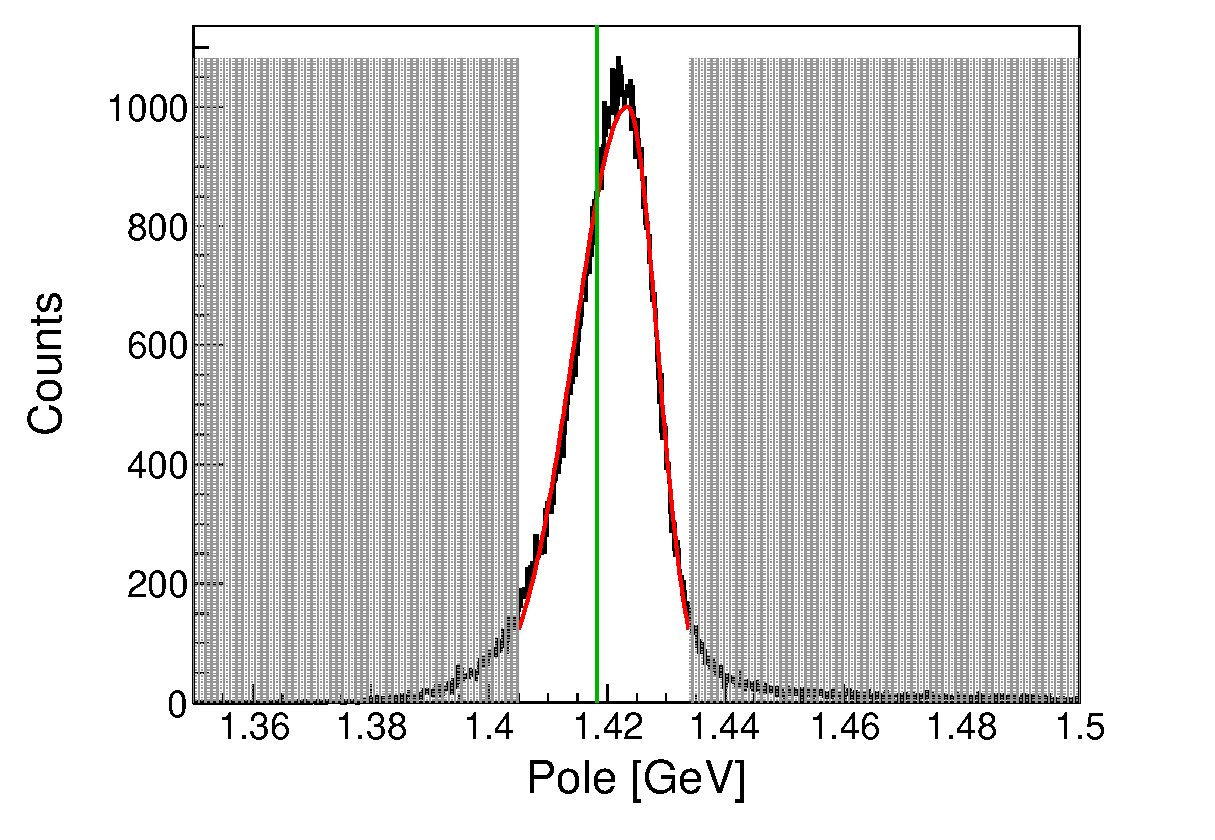
\includegraphics[width=4cm]{../pic/Dron/fit_L1405_pole_KzeroN_4.eps}
    \end{minipage}
  \end{tabular}

  \begin{tabular}{ccc}
    \begin{minipage}{0.33\hsize}
      \includegraphics[width=4cm]{../pic/Dron/fit_L1405_pole_Kmp_3.eps}
    \end{minipage}
    \begin{minipage}{0.33\hsize}
      \includegraphics[width=4cm]{../pic/Dron/fit_L1405_pole_KN_3.eps}
    \end{minipage}
    \begin{minipage}{0.33\hsize}
      \includegraphics[width=4cm]{../pic/Dron/fit_L1405_pole_KzeroN_3.eps}
    \end{minipage}
  \end{tabular}

  \begin{tabular}{ccc}
    \begin{minipage}{0.33\hsize}
      \includegraphics[width=4cm]{../pic/Dron/fit_L1405_pole_Kmp_2.eps}
    \end{minipage}
    \begin{minipage}{0.33\hsize}
      \includegraphics[width=4cm]{../pic/Dron/fit_L1405_pole_KN_2.eps}
    \end{minipage}
    \begin{minipage}{0.33\hsize}
      \includegraphics[width=4cm]{../pic/Dron/fit_L1405_pole_KzeroN_2.eps}
    \end{minipage}
  \end{tabular}

  \begin{tabular}{ccc}
    \begin{minipage}{0.33\hsize}
      \includegraphics[width=4cm]{../pic/Dron/fit_L1405_pole_Kmp_1.eps}
    \end{minipage}
    \begin{minipage}{0.33\hsize}
      \includegraphics[width=4cm]{../pic/Dron/fit_L1405_pole_KN_1.eps}
    \end{minipage}
    \begin{minipage}{0.33\hsize}
      \includegraphics[width=4cm]{../pic/Dron/fit_L1405_pole_KzeroN_1.eps}
    \end{minipage}
  \end{tabular}
  
  \begin{tabular}{ccc}
    \begin{minipage}{0.33\hsize}
      \includegraphics[width=4cm]{../pic/Dron/fit_L1405_pole_Kmp_0.eps}
    \end{minipage}
    \begin{minipage}{0.33\hsize}
      \includegraphics[width=4cm]{../pic/Dron/fit_L1405_pole_KN_0.eps}
    \end{minipage}
    \begin{minipage}{0.33\hsize}
      \includegraphics[width=4cm]{../pic/Dron/fit_L1405_pole_KzeroN_0.eps}
    \end{minipage}
  \end{tabular}
  
  \caption{
    This figure shows the distribution and fit of the poles of $\Lambda(1405)$, generated using Gaussian random numbers.
    The right, center, and left panels correspond to the results based on the $K^- p$, $\bar{K}N$, and $K^0 n$ thresholds, respectively.
    The top row represents the fit over the entire range,
    followed by rows corresponding to the equivalent ranges of $3\sigma$, $2.5\sigma$, $2\sigma$, $1.5\sigma$, and $1\sigma$.
    The fit results are shown as red lines, with gray hatched areas representing regions excluded from the fit.
    The green lines indicate the pole positions corresponding to the best-fit values shown in Figure \ref{fig:fit_2step_I0}.
  }
  \label{fig:fit_L1405_pole}
\end{figure}
